\documentclass[a4paper,12pt,oneside, tikz]{book}  
\usepackage[utf8]{inputenc}
\usepackage{tcolorbox}
\usepackage{amsmath,amssymb,amsthm, enumitem, hyperref, tabto} 
\usepackage[T1]{fontenc}
\usepackage[utf8]{inputenc}
\usepackage[english]{babel}
\usepackage{wrapfig}
\usepackage{lastpage}
\usepackage{tikz}
\usetikzlibrary{external}
\tikzexternalize % activate!
\usepackage[american]{circuitikz}
\usepackage[absolute,overlay]{textpos}
\usepackage[left=2cm,right=2cm]{geometry}
\usepackage[english]{babel}
\usepackage{fancyhdr}
\usepackage{float}
\hypersetup{
    colorlinks=true,
    linkcolor=blue,
    filecolor=magenta,      
    urlcolor=cyan,
    pdftitle={Studio 4},
    pdfpagemode=FullScreen,
    }

\urlstyle{same}
\usepackage{xcolor}
\usepackage{colortbl}

\usepackage{graphicx, multicol, latexsym}
\usepackage{blindtext}
\usepackage{subfigure}
\usepackage{caption}
\usepackage{capt-of}
\usepackage{tabu}
\usepackage{booktabs}

\usepackage{fancyhdr}            % Permits header customization. See header section below.
\fancypagestyle{plain}{
    \lhead{}
    \fancyhead[R]{\thepage}
    \fancyhead[L]{}
    \renewcommand{\headrulewidth}{0pt}
    \fancyfoot{}
}

\pagestyle{fancy}
\fancyhead[R]{\thepage}
\fancyhead[L]{}
\renewcommand{\headrulewidth}{0pt}
\fancyfoot{}

\usepackage{array}
\newcolumntype{P}[1]{>{\centering\arraybackslash}p{#1}}

\usepackage{titlesec}

\titleformat{\chapter}[display]{\normalfont\huge\bfseries}{\chaptertitlename\ \thechapter}{20pt}{\Huge}

% this alters "before" spacing (the second length argument) to 0
\titlespacing*{\chapter}{0pt}{0pt}{40pt}


\addto\captionsenglish{\renewcommand{\chaptername}{Activity}} 


\title{\textbf{DC Motors} Studio Report \\ CG1111A Studio 7}

\author{Prannaya Gupta (B02)}

\begin{document}

\maketitle

\chapter{}

My last two digits are "67", thus as per the given formula, by Parameter Set Number is \textbf{18}. Running the simulator, we get the following table:

\begin{table}[H]
    \centering
    \begin{tabular}{|c|c|}
         \hline Motor Voltage $V_m$ (V) & Rotational Speed N (RPM)  \\
         \hline 7 & 691 \\
         8 & 1043 \\
         9 & 1354 \\
         10 & 1666 \\
         11 & 1981 \\
         12 & 2450 \\
         \hline
    \end{tabular}
    \caption{Simulated Readings}
    \label{tab:activity1}
\end{table}

For this studio, we note that $\omega = \frac{2\pi}{60}N$, thus the equation $\omega = \frac{V_m}{K_e} - \frac{R_mI_m}{K_e}$ is really just a linear line. Therefore, we use the linear trendline.

\begin{figure}[H]
    \centering
    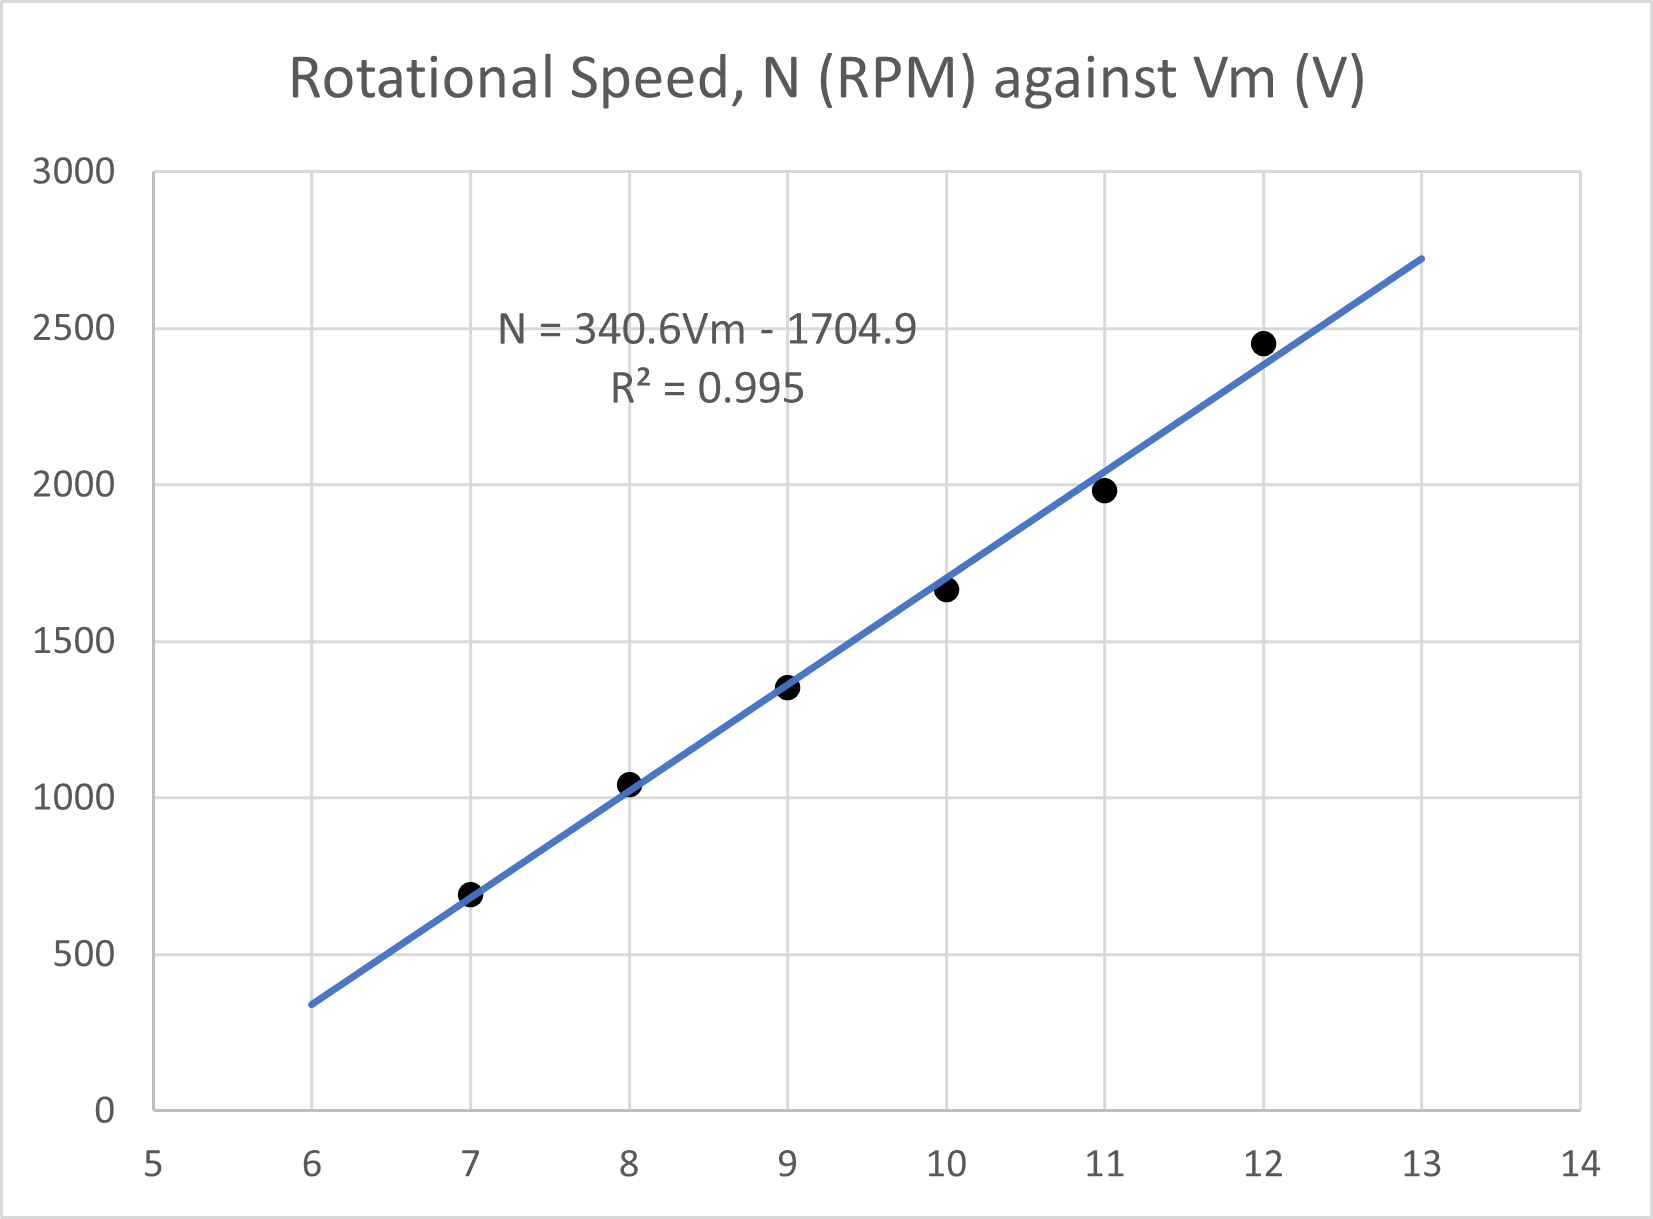
\includegraphics[width=0.6\textwidth]{images/activity1graph.png}
    \caption{Graph of Rotational Speed, $N$ (RPM) against Motor Voltage, $V_m$}
    \label{fig:activity1graph}
\end{figure}

From here, we get that the equation of the curve is:
$$N = 340.6V_m - 1704.9$$

The motor does not start turning immediately after the voltage is applied is because 

\chapter{DC Motor Characterization}
\begin{table}[H]
    \centering
    \begin{tabular}{|c|c|c|c|}
         \hline Torque Load & Motor Current $I_m$ (A) & Rotational Speed N (RPM) & $\omega$ (rad/s)  \\
         \hline $\sim$2/3 of slider & 0.769 & 861 & 90.16 \\
         $\sim$1/2 of slider & 0.581 & 1530 & 160.22 \\
         $\sim$1/3 of slider & 0.410 & 2450 & 256.56 \\
         $\sim$1/6 of slider & 0.204 & 3212 & 336.36 \\
         $\sim$1/10 of slider & 0.128 & 3444 & 360.65 \\
         \hline
    \end{tabular}
    \caption{Simulated Readings}
    \label{tab:activity2}
\end{table}

The following represents

\end{document}